\chapter{Photoinjection of Charge Carriers}
% \label{chap:conclusion}



\section{Different Disorders}

\begin{figure}[h!] % можно [t], [b], [p], [h]
    \centering
    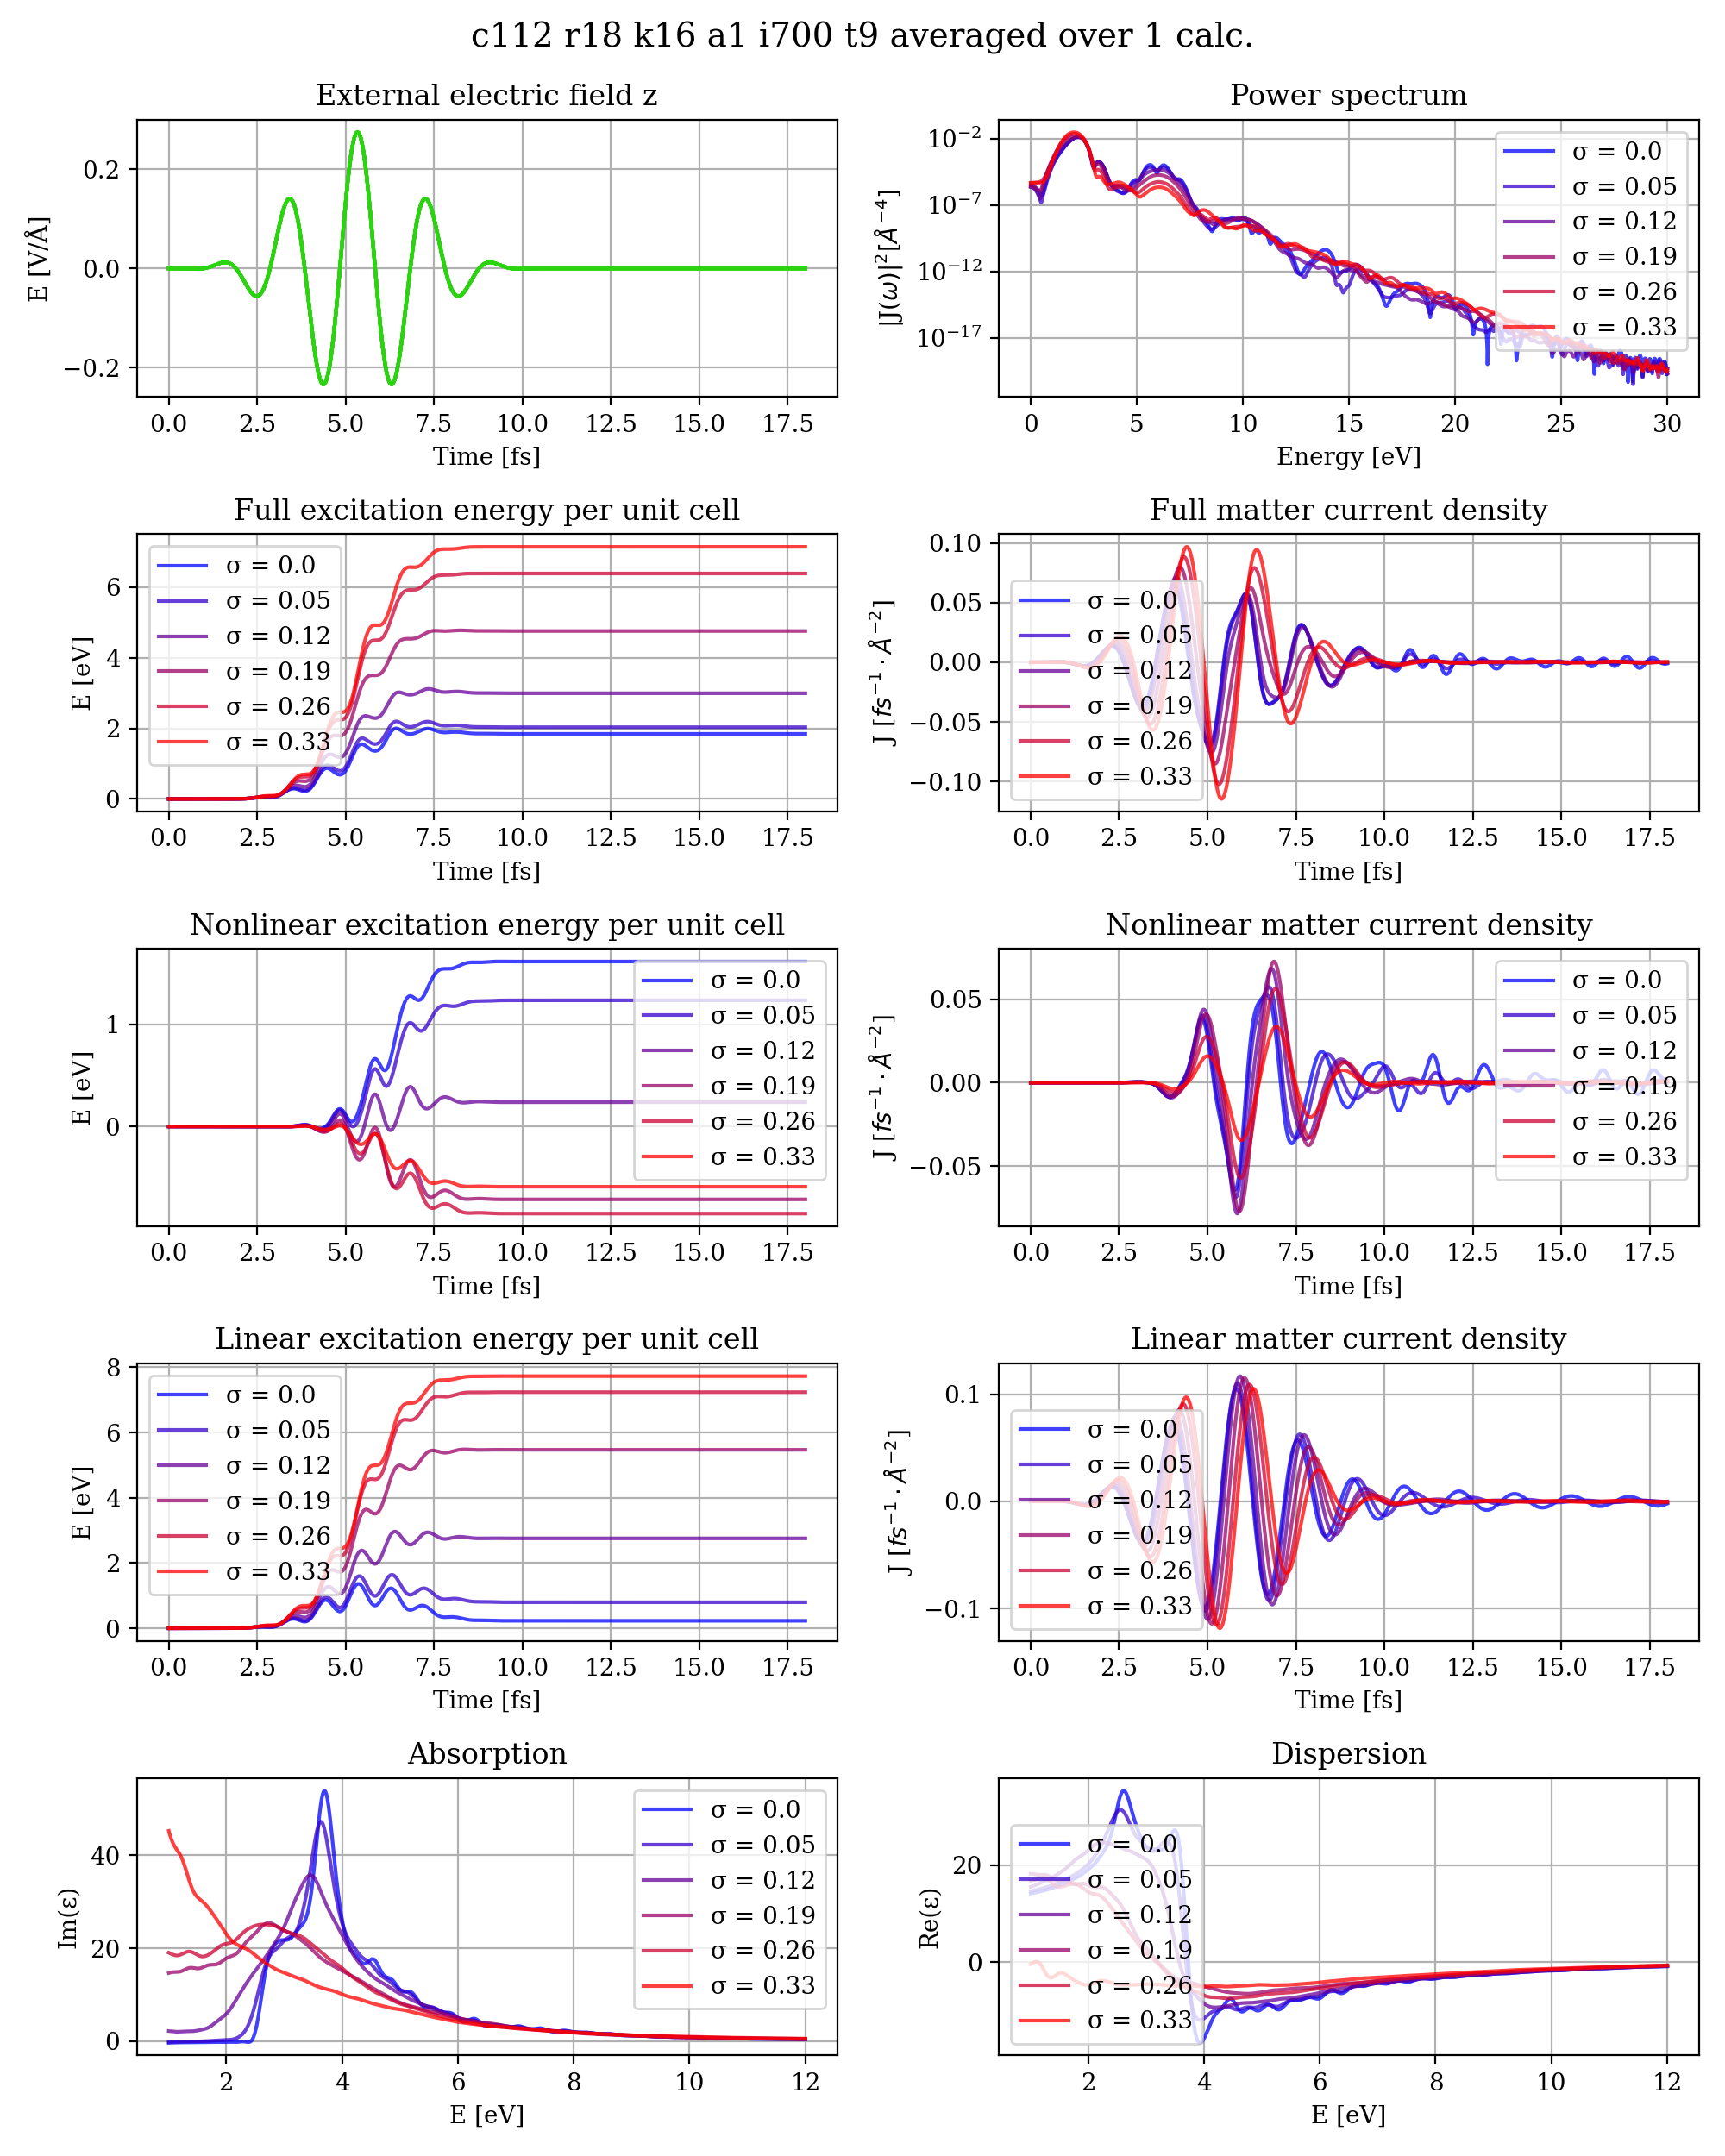
\includegraphics[width=0.72\linewidth]{figures/disorder_comparison_Jul22.png} % путь к файлу
    \caption{Energy and current characteristics for different degrees of disorder. Mean energy in the pump pulse is 1 eV.}
    \label{fig:myimage}
\end{figure}

From the absorption graphs we see that the band gap is decreasing, as predicted by Eq. \ref{eq:rho_final}. But from some point on, at low energies, we get an incorrect contribution due to the broadening caused by the finite length of the time window in which the calculation takes place. This problem can be solved by taking several time windows of increasing size and then taking the common part as the correct one. However, for modeling defects, when the zone width decreases by about 0.1 eV, the accuracy is sufficient for us.

As can be seen, the band gap narrows very strongly with increasing disorder, so that linear transitions become dominant, which make the main contribution to the photoinjection energy.

A phase lag in the current is also clearly visible as disorder increases. This can be explained by several considerations:
\begin{itemize}
\item \textbf{Localization of states:}
        Electron states become increasingly localized. The current becomes polarized and hopping, introducing a delay in the response.
\item \textbf{Increase of $m_{eff}^*$:}
        Due to the decrease in the band gap, more and more transitions become accessible, which leads to an increasingly wider population of the conduction band, which leads to a significant increase in the effective mass as can be seen from \cite{Qasim_2018}, which leads to a delay.
\end{itemize}

However, these data should be treated with a little skepticism since the cell size is small and it is quite possible that the current attenuation would occur faster.

\section{Population of the Conduction Band}
\textcolor{red}{TO DO}